\documentclass[a4paper,french]{article}
\usepackage{rfiap2018_resume}

\usepackage[utf8]{inputenc}
\usepackage[T1]{fontenc}
\usepackage{babel}
\usepackage{times, fourier}

\usepackage{array}
\newcolumntype{x}[1]{>{\centering\let\newline\\\arraybackslash\hspace{0pt}}p{#1}}
\usepackage{tabulary}
\usepackage{booktabs}
\usepackage{multirow}


\usepackage{siunitx}

\usepackage{standalone}

\usepackage{enumitem}

\usepackage{graphicx}
\usepackage{subfig}
\usepackage{floatrow}
\usepackage[figurename=Fig., tablename=Tab.]{caption}
\captionsetup{labelsep=period}

\newcounter{SubFigCounter}
\setcounter{SubFigCounter}{1}

\begin{document}
    \date{}
    \title{
        \Large\bf Autoqualification de modèle $3D$ de bâtiments pour l'évaluation de méthode de reconstruction.
    }
    \author{
        \begin{tabular}[t]{c@{\extracolsep{4em}}c@{\extracolsep{4em}}c@{\extracolsep{4em}}c}
            Oussama Ennafii${}^1$ & Clément Mallet${}^1$ & Arnaud Le-Bris${}^1$ & Florent Lafarge${}^2$ \\
        \end{tabular}
        {}\\
        \\
        ${}^1$        Univ. Paris-Est, LaSTIG MATIS, IGN, ENSG, 94160 Saint-Mandé, France\\
        ${}^2$        Inria, Titane, 06902 Sophia Antipolis, France
        {}\\
        \\
        oussama.ennafii@ign.fr\\
    }
    \maketitle
    \thispagestyle{empty}

    \section{Introduction}
    \begin{itemize}
        \item Les modèles $3D$ urbains ont un champs d'application~\cite{Biljecki2015} (\textit{c.f.} Table~\ref{tab::3d_applications}).
        \item La reconstruction automatique de scènes urbaines est l'objet d'intérêt de la communauté scientifique autant que les industriels\cite{Musialski2012}.
        \item Même les derniers algorithmes de modélisation automatiques urbaines ne sont pas viables du point de vue opérationel.
        \item Exemple opérationnel: la solution à l'IGN~\cite{taillandier2004reconstruction,Taillandier2004, Durupt2006} industrialisée sous le nom Bati3D, requiert autant d'effort des opérateurs que de saisir les surfaces à la main.
    \end{itemize}

    \begin{table}[h!]
        \begin{center}
            \begin{tabular}{l l l}
                \toprule
                Planification & Simulation & Visualisation \\
                \midrule
                Plannification urbaine & Microclimat & Architecture \\
                Intervention d'urgence & Propagation d'onde
 & Cadastre \\
                Décoration d'intérieur & Ruisselement d'eau & Tourisme \\
                Réseau de communication & Intervention armée & Jeux video \\
                \bottomrule
            \end{tabular}
            \caption{\label{tab::3d_applications} Bref recensement des applications des modèles $3D$ urbains~\cite{Biljecki2015, Scholze2002}.}
        \end{center}
    \end{table}

    Les méthodes de diagnostique prédictives permettrons:
    \begin{itemize}
        \item la détection de changement.
        \item la correction des modèles urbains.
        \item l'évaluation, et ainsi la sélection, d'algorithmes de revonstruction urbaines.
        \item l'évaluation de la qualité de reconstruction par la foule.
    \end{itemize}

    Les contributions majeures:
    \begin{itemize}
        \item Une nouvelle taxonomie est considérée pour hiérarchiser les erreurs qui peuvent affecter les modèles $3D$ de bâtiments. Elle est indépendente des démarches de reconstruction $3D$ et flexibles quant aux différents types de modèles en entré.
        \item La qualification est donc formulée comme un problème de classification supervisée.
        \item Une référence d'attributs est calculée à partir de la géométrie du modèle de bâtiments en entrée. Des attributs basés sur la comparaison avec les orthoimages ou le Modèle Numérique de surface.
    \end{itemize}
    \section{\'Etat de l'art}
    On peut classifier les méthodes d'évaluation de modèles urbains selon deux critères:
    \begin{itemize}
        \item le type de sortie: macro-indices géométriques, erreurs topologiques ou géométriques. Les indices géométriques peuvent résumer la précision d'une modélisation mais ne permettent pas de bien décrire les erreurs: un simple maillage $3D$ de points LiDAR ou de MNS donneront une meilleur reconstruction dans ce cas~\cite{rottensteiner2014results}. Une taxonomie d'erreurs pourrait palier à ce déficit mais peut, par contre, facilement être surajustée à une scène ou aux données d'entrées.
        \item le type de données de référence: Modèle de très grande précision géométriques, données issu de la photogrammétrie ou modèles de classification. Les modèle urbains de grands précisions ne sont pas facile à acquérir. Même si elles sont indépendentes des modèles à qualifier, il n'est pas facile d'en produire assez, en grande variété, afin de bien évaluer les méthodes de reconstruction. Les données photogrammétriques, étant non structurées, ne permettent pas, de leur part, de relever les erreurs sémantiques~\cite{Akca2010}. Les modèles de classification sont bien moins couteux en ressources pour prédire la qualité des modèles urbains. Ils sont, en revanche, aussi potent que la taxonomie d'erreurs sur laquelle repose la classification.
    \end{itemize}

    \begin{itemize}
        \item \cite{Henricsson1997} extrait des indices de complétude, précision géométrique et disparité de forme. Ces indices sont calculés à partir de modèle $3D$ de référence acquis manuellement avec $\pm \SI{10}{\cm}$ d'erreur estimée.
        \item En analysant les sources d'erreurs dans les méthodes de modèlisation urbaines, \cite{Voegtle2003} propose deux indices géomètriques: précision de position et de hauteur. Les données sont aussi construit à partir de mesures géodésiques d'erreurs relatives de $\pm \SI{5}{\cm}$.
        \item \cite{Zeng2014} propose une estimation de précision du modèle urbain en comparant, par rapport à un modèle manuellement reconstruit, les écarts de volume, les différences entre surfaces en utilisant l'expansion SPHARM~\cite{brechbuhler1995parametrization} et l'écart positionel de points d'intérêts.
        \item \cite{Kaartinen2005} compare des mesures de position et de distance sur des points d'intérêts ainsi que les inclinaisons de toit de bâtiments avec des données de références de pécision estimée à $\vert\vert \sigma_{xy} \vert\vert \leq \SI{8.3}{\cm} \text{ et } \vert \vert \sigma_z \vert\vert \leq \SI{3.5}{\cm}$
        \item \cite{Akca2010} utilise les nuages de points LiDAR pour sortir trois types d'erreurs: systématique, grossière ou aléatoire. Les erreurs systématiques proviennent de la différences de systèmes de références et de position de bâtiments individuels. Les erreurs de complétudes relèvent les parties manquantes d'un bâtiments reconstruit alors que les erreurs aléatoire résultent du bruit intrinsèque des capteurs.
        \item \cite{OudeElberink2010} propose aussi de comparer les modèles de reconstructions aux points LiDAR. Ils relèvent, ainsi, visualement des erreurs sémantiques --- ou topologiques --- en comparant et analysant les résiduels tridimensionnels du modèle et les points LiDAR correspondants.
    \end{itemize}

    \begin{itemize}
        \item \cite{Boudet2006} propose un nouveau cadre d'étude, où la qualification se résume à une prédiction d'erreurs à partir d'un modèle de classification préentraîné. La taxonomie proposée repose sur le paradigme des feux de circulation: Correct, acceptable, généralisé et faux. Chaque erreur correspond à un degré de confiance de l'exactitude du modèles à classer. Les attributs sont calculés à partir des images orientées. On calcule des indices de cohérence de texture de facettes, en mesurant la corélation entre images orientées, et des indices de cohérence structurelle, en comparant les segements 3D extraits des images avec le modèle d'entrée. En se basant sur les indices ainsi calculer des seuils sont définis pour décider de la qualité du model (i.e. arbre de décision).
        \item \cite{Michelin2013} porpose quant à lui une taxonomy basée sur les défault topologique ou géométrique qui peuvent affecter des modèles de niveau de détail $LoD2$~\cite{kolbe2005citygml}. La catégorisation des erreurs étudiée dans \cite{Michelin2013} adopte le point de vue des méthodes de reconstruction. Elle différencie entre les erreurs d'empreinte, qui proviendrait des données d'entrées de la modélisation, les erreurs de reconstruction intinsèques à la méthode et une erreur due à l'occlusion végétale. Neuf erreurs, en total, sont relevées: Erreurs d'empreinte (contour erroné, bâtiment inexistant, cours intérieur manquante et empreinte imprécise), erreurs de reconstruction (sous-segmentation, sur-segmentation, toit inexact, translation en Z) et erreurs de végétation. Les attributs calculés sont calculés à partir de segments $3D$ extrait des images orientées, ou à partir de MNS. Ces segments 3D seront comparés aux segments du modèles à classifier. Les attributs sont extraits aussi à travers l'angle de vue du ciel ou encore du masque NDVI.
    \end{itemize}

    \section{Taxonomie d'erreurs}

    La taxonomie proposée regroupe les erreurs rencontrées selon l'échelle d'étude.
    \begin{itemize}
        \item une famille d'erreurs est consacrée aux défauts qui affectent le bâtiment en entier. Cela corresponderais à un niveau de détail $LoD 0\cup LoD 1$. Elle est nommée: \emph{Erreurs de Bâtiment}.
        \item une famille contient les erreurs qui concernent les facettes --- façades ou toit --- du bâtiments (niveau $LoD 2$): \emph{Erreurs de Facettes}.
        \item une famille englobe les erreurs qui éteignent les mircrostructures reconstruites (niveau $LoD 3$): \emph{Erreurs de Microstructures}.
        \item Du point de vue opérationnel, pas tout les bâtiments sont qualifiables. C'est ainsi qu'une famille est elle créée pour rassembler ces types d'erreurs: \emph{Bâtiments non qualifiables}.
    \end{itemize}

    Cette catégorisation reste indépendente de la méthode de reconstruction ou de la scène à modéliser.
    \begin{itemize}
        \item On cherche un étiquetage non redondant: les erreurs à relever doivent rester indépendentes entre elles au maximum et ne représenter que des déficiences particulères. On dira que ce sont des erreurs \emph{atomiques}.
        \item Les erreurs peuvent être d'ordre topologique ou géométrique. Les erreurs topologiques relèvent les défauts de structure du modèle reconstruit. Les erreurs géométriques mettent en évidence les défauts d'imprécision de la reconstruction.
        \item On attribut pour chaque erreur atomique une note sur une échelle de $0$ à $10$. Elle représente le degré de confiance en la présence du défaut. Cela revient à une discrétisation de la probabilité d'existence de l'erreur.
    \end{itemize}

    Nous appliquons cette approche à une surface de $\SI{0.2}{\km \squared}$ contenant $502$ bâtiments dans la ville d'\'Elancourt. C'est une région résidentielle dense qui comprends surtout des bâtiments à deux pans de toit, une école au Nord Ouest du quartier et une station-service au Sud. Les modèles d'entrées sont générés à partir d'une version industrialisée de~\cite{Durupt2006}. La méthode repose que une base de données d'empreinte de bâtiments (cadastrales ou autes) et l'extrapolation de la topologie du toit. Les toits simulés à partir des images orientées sont confrontés au MNS à $\SI{6}{\cm}$ de résolution. Les façades du modèle relie la line de goutière aux sol. On obtient une modélisation $2.5D$ de la scène à un niveau de détail $LoD 2$.

    Confronté à cette base de données, on relève les erreurs suivantes:

    \begin{enumerate}[label= (\roman*).]
        \item Bâtiments non qualifiables (\textit{c.f.} Figure~\ref{fig::samples}\ref{fig::unq_bul}):
        \begin{itemize}
            \item Bâtiment incomplet: seul une partie du bâtiment est modélisée,
            \item Bâtiment modifié: le bâtiment modéliser a changé est ne peut être qualifier,
            \item Occlusion: le bâtiment est caché par de la végétaion ou autre,
            \item Inconnu: Forme inconnue impossible à qualifier sans vérification sur le terrain;
        \end{itemize}
        \item Erreurs de Bâtiment (\textit{c.f.} Figure~\ref{fig::samples}\ref{fig::bul_err}):
        \begin{itemize}
            \item Sous segmentation: deux bâtiments, ou plus, représentés comme un seul,
            \item Sur segmentation: un bâtiments est modélisé en deux ou plusieurs bâtiments,
            \item Empreinte Imprécise: l'empreinte du bâtiment défectueuse,
            \item Hauteur Imprécise: hauteur de bâtiment mal estimée;
        \end{itemize}
        \item Erreurs de Facette (\textit{c.f.} Figure~\ref{fig::samples}\ref{fig::fac_err}):
        \begin{itemize}
            \item Sous segmentation: deux facettes, ou plus, représentés comme un seul,
            \item Sur segmentation: un facettes est modélisé en deux ou plusieurs bâtiments,
            \item Segmentation imprécise: les arrêtes qui séparent les facettes sont inexactes,
            \item Pente Imprécise: pente inexacte.
        \end{itemize}
    \end{enumerate}

    \thisfloatsetup{heightadjust=object}
    \begin{figure}[h!]
        \begin{center}
            \ffigbox{
                \ffigbox[\FBwidth]{
                    \begin{subfloatrow}[4]
                        \captionsetup{labelformat=brace, justification=raggedright}
                        \ffigbox[\FBwidth]{\caption{Half Building: only a portion of the building is reconstructed.}\label{fig::half_building}}{\fbox{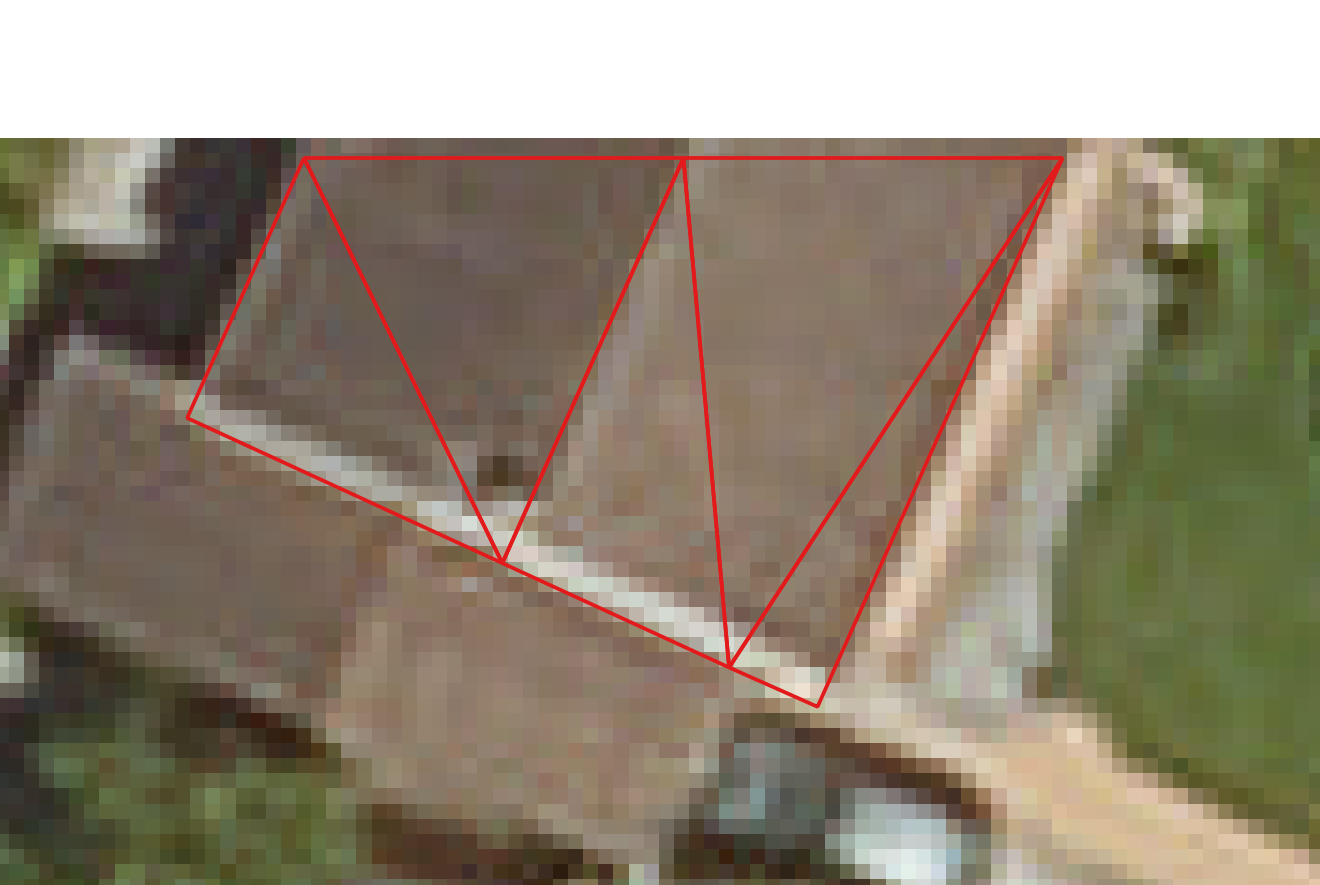
\includegraphics[width=.24\textwidth]{images/raster/Unqualified_Errors/half_building}}}
                        \ffigbox[\FBwidth]{\caption{Changed Building: the building has changed so we cannot qualify it.}\label{fig::changed}}{\fbox{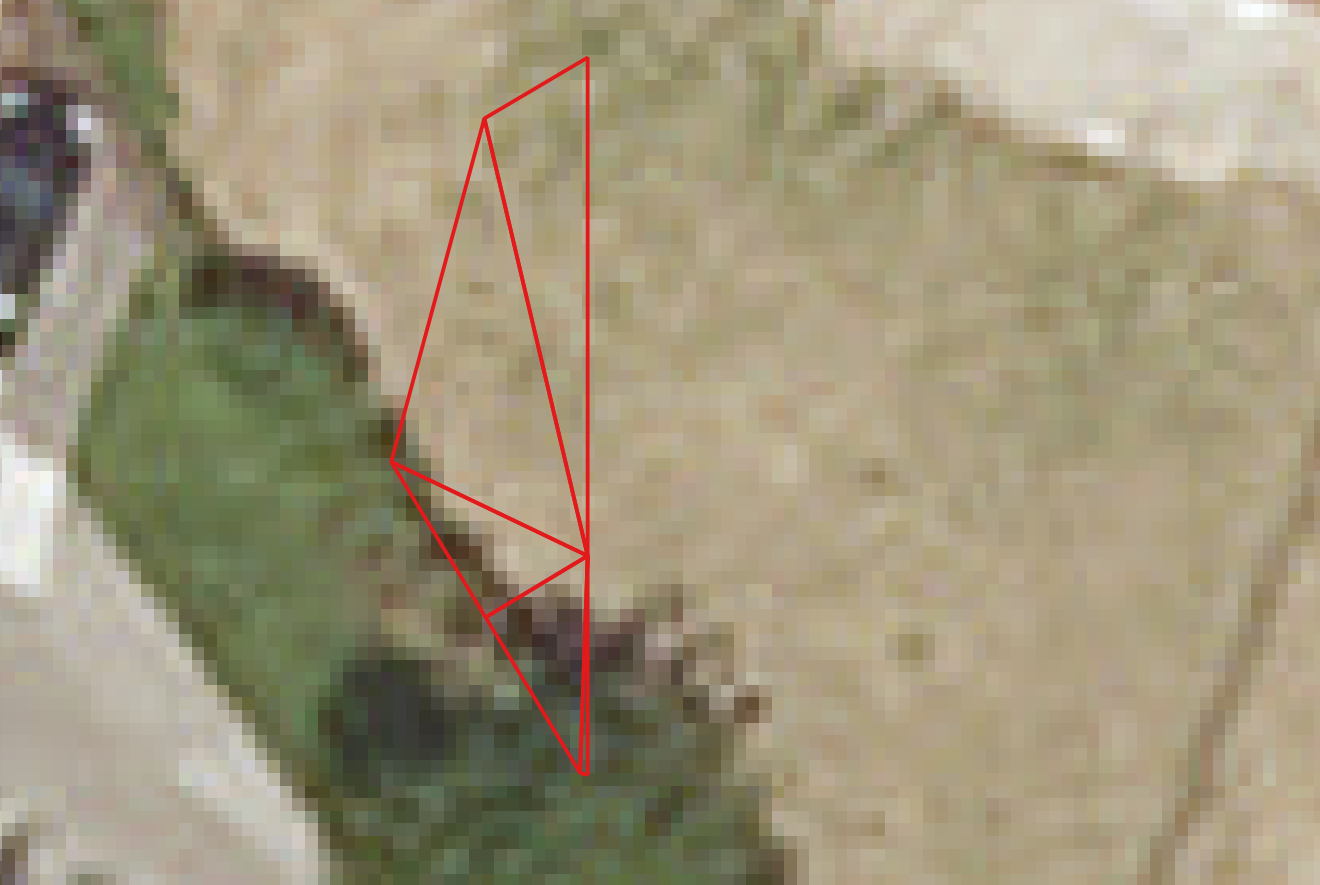
\includegraphics[width=.24\textwidth]{images/raster/Unqualified_Errors/changed}}}
                        \ffigbox[\FBwidth]{\caption{Occlusion: the building is occluded by vegetation here.}\label{fig::occlusion}}{\fbox{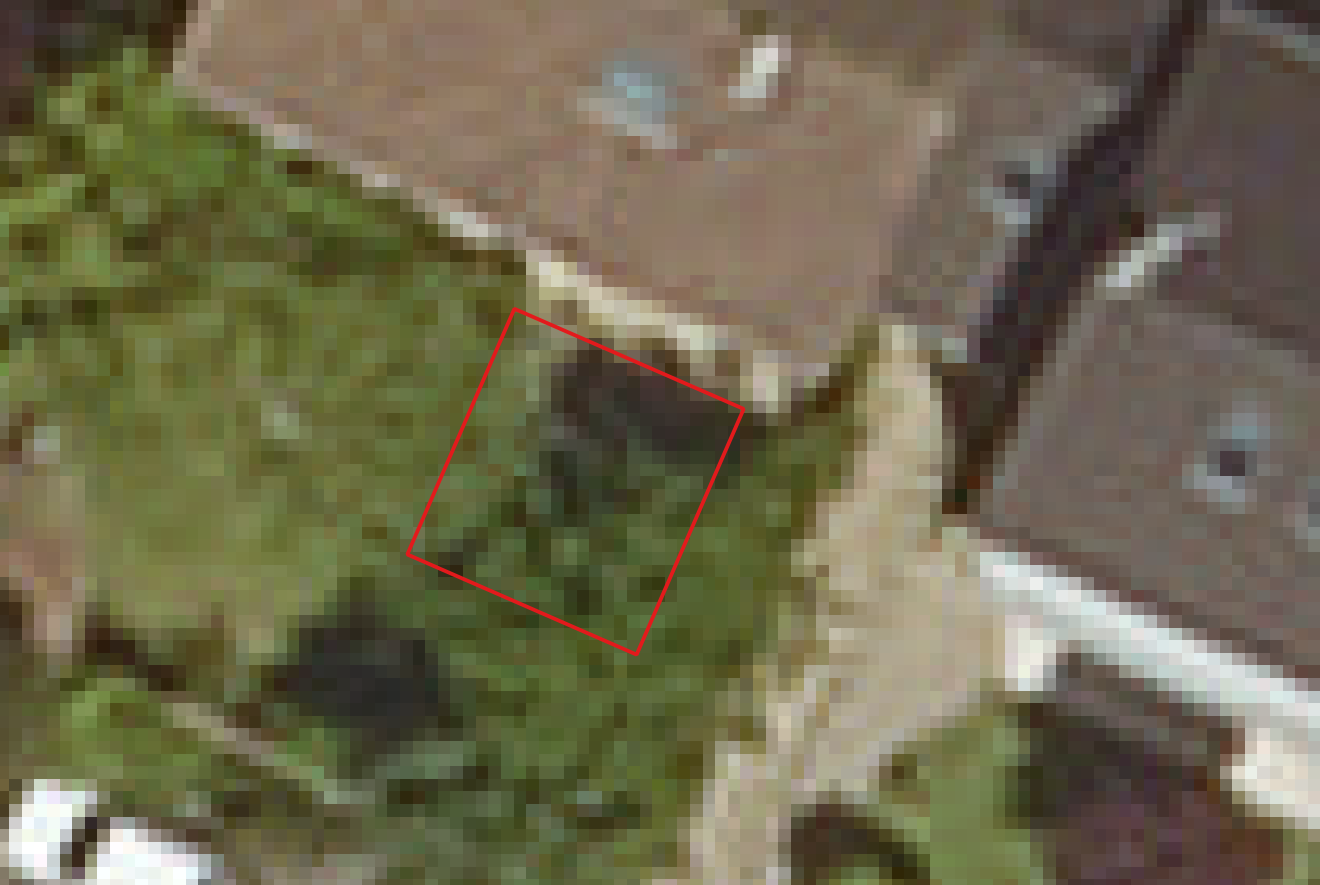
\includegraphics[width=.24\textwidth]{images/raster/Unqualified_Errors/occlusion}}}
                        \ffigbox[\FBwidth]{\caption{Unknown: Unknown shape that cannot be verified on the ground.}\label{fig::unknown}}{\fbox{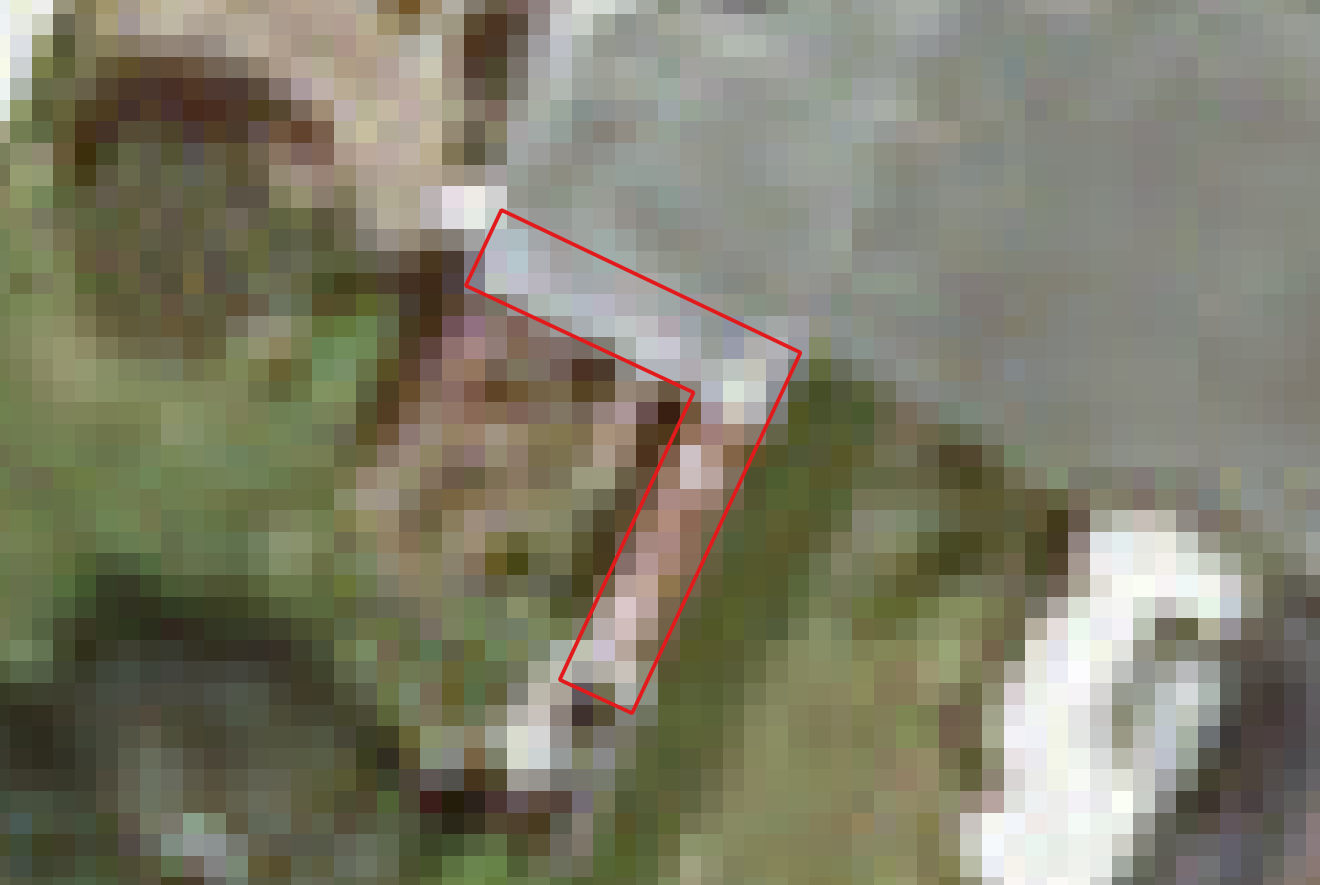
\includegraphics[width=.24\textwidth]{images/raster/Unqualified_Errors/unknown}}}
                    \end{subfloatrow}
                }
                {
                    \renewcommand\figurename{}
                    \renewcommand{\thefigure}{(\roman{SubFigCounter})}

                    \caption{Unqualified building errors samples.}\label{fig::unq_bul}
                    \refstepcounter{SubFigCounter}
                }
                \ffigbox[\FBwidth]
                {
                    \begin{subfloatrow}[4]
                        \captionsetup{labelformat=brace, justification=raggedright}
                        \ffigbox[\FBwidth]{\caption{Under Segmentation: Two or more buildings grouped into one.}\label{fig::under_bul}}{\fbox{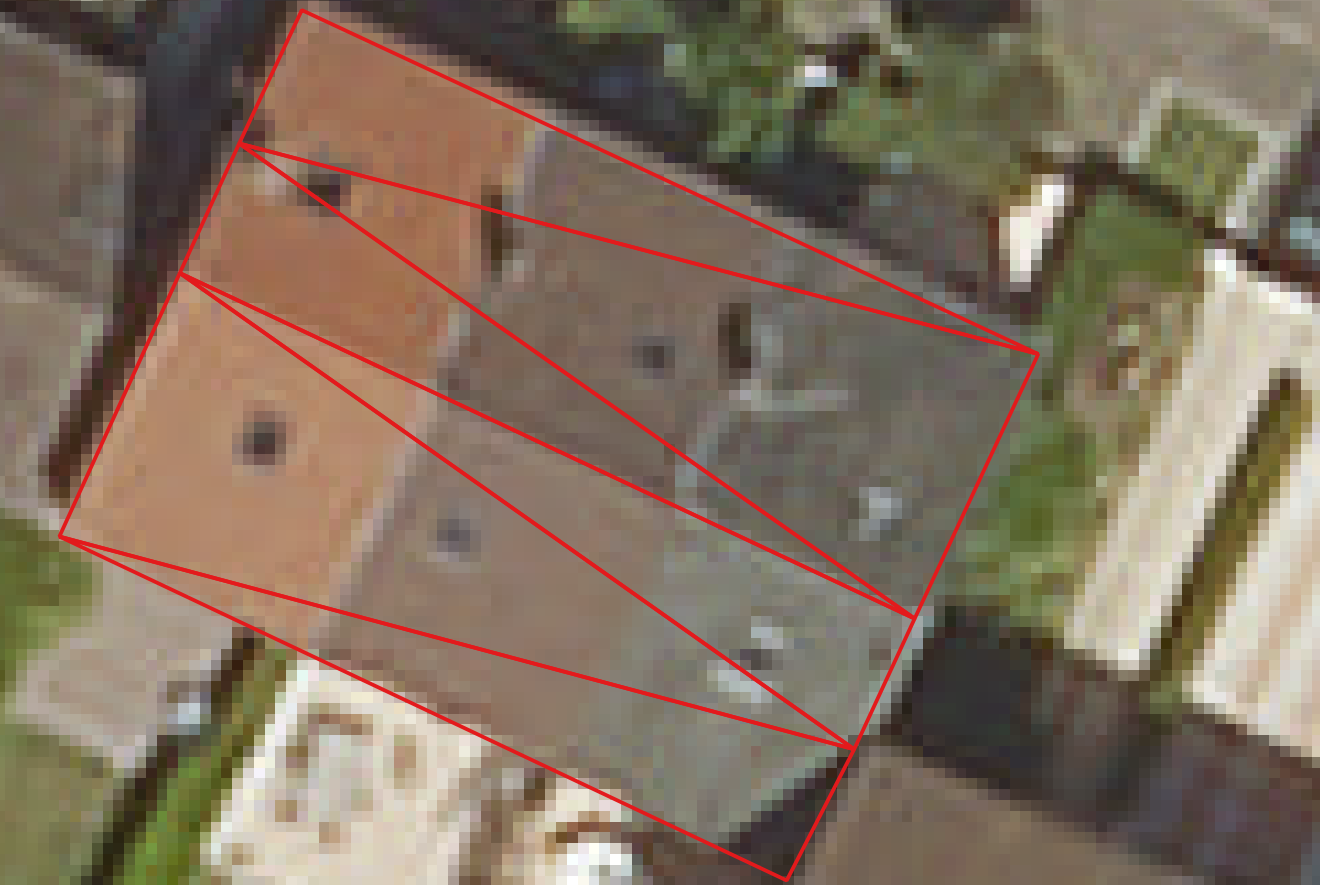
\includegraphics[width=.24\textwidth]{images/raster/Building_Errors/under_segmentation}}}
                        \ffigbox[\FBwidth]{\caption{Over segmentation: One building segmented into two or more buildings.}\label{fig::over_bul}}{\fbox{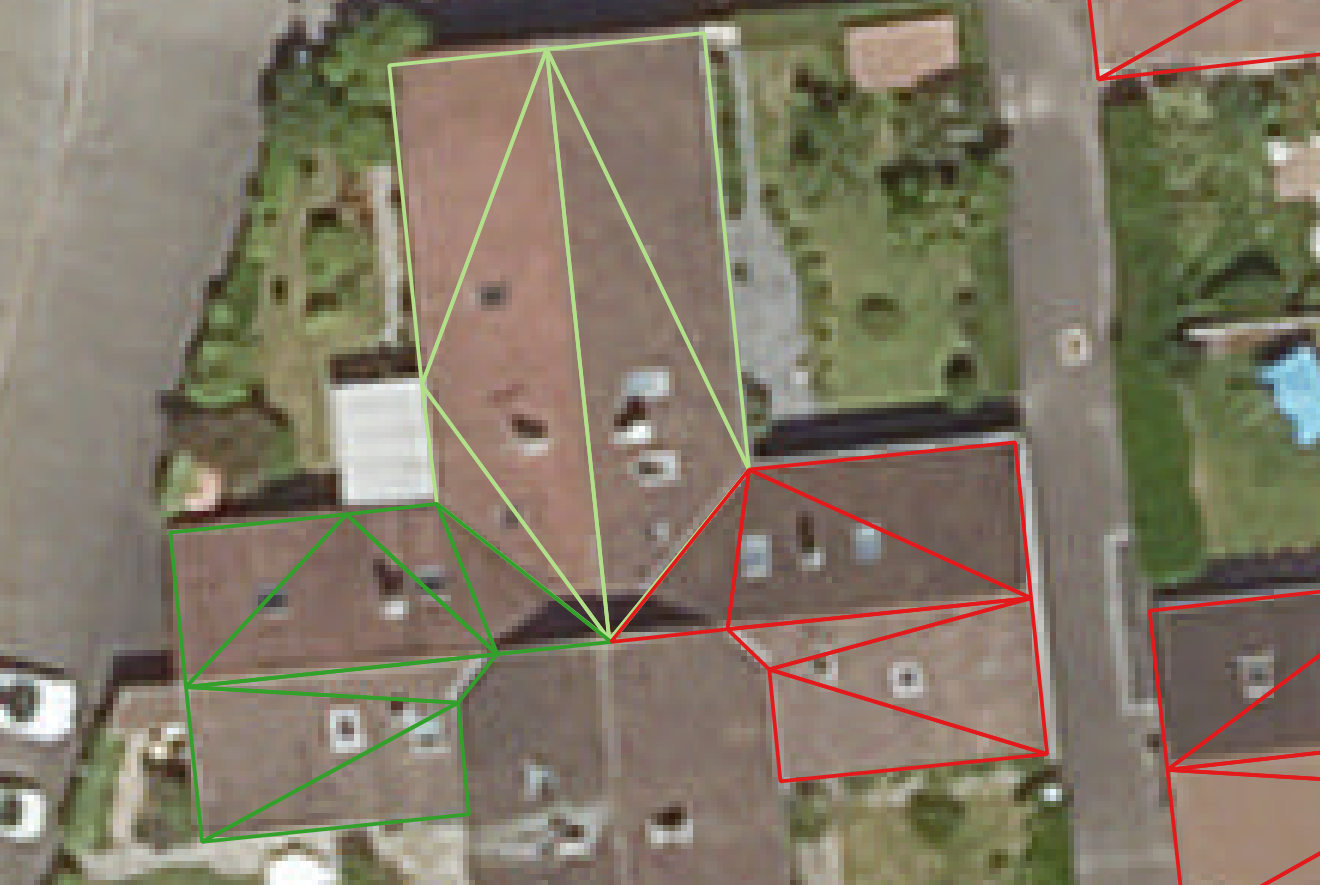
\includegraphics[width=.24\textwidth]{images/raster/Building_Errors/over_segmentation}}}
                        \ffigbox[\FBwidth]{\caption{Footprint: Wrong building footprint.}\label{fig::footprint}}{\fbox{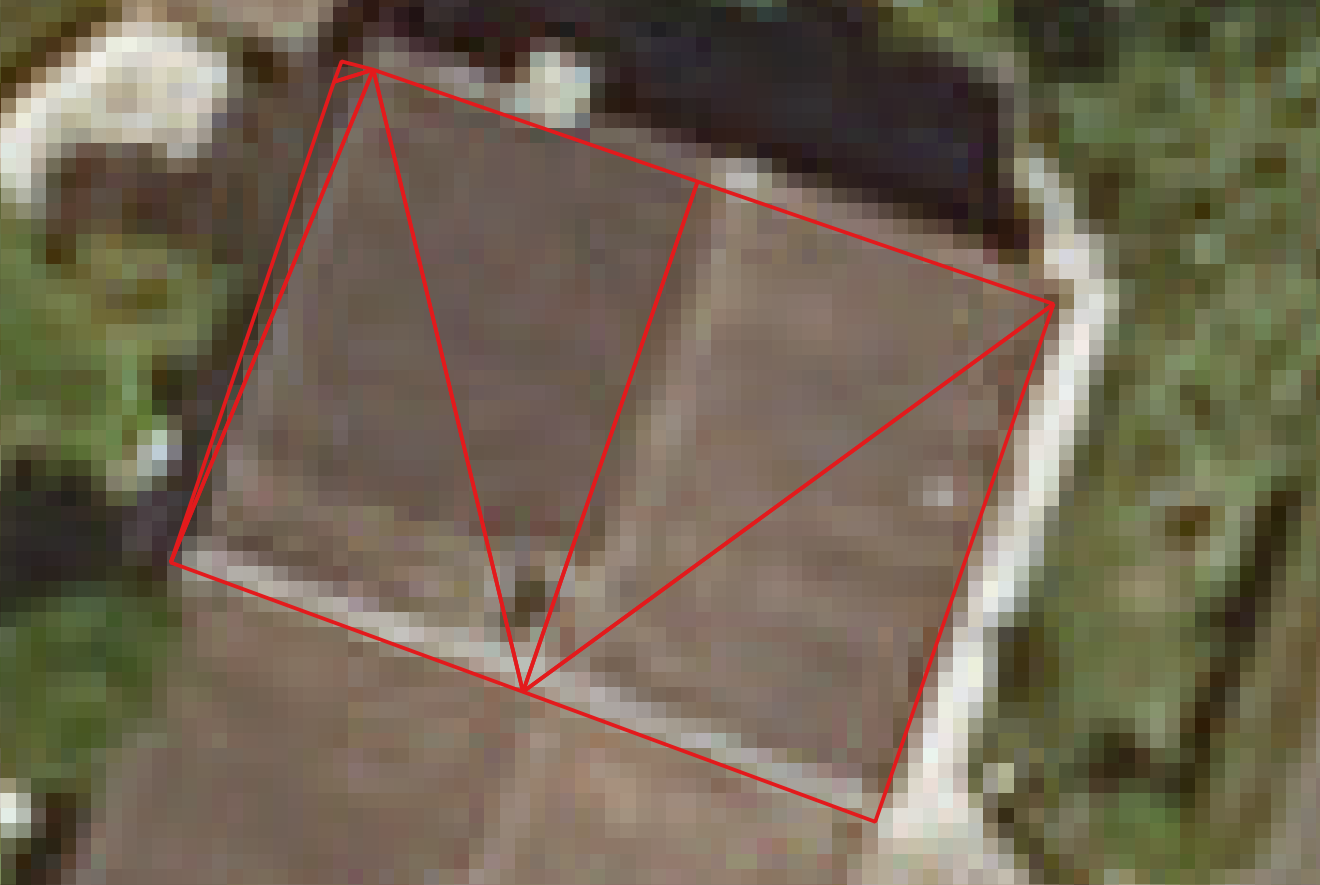
\includegraphics[width=.24\textwidth]{images/raster/Building_Errors/footprint}}}
                        \ffigbox[\FBwidth]{\caption{Height: Wrong building height.}\label{fig::too_low}}{\fbox{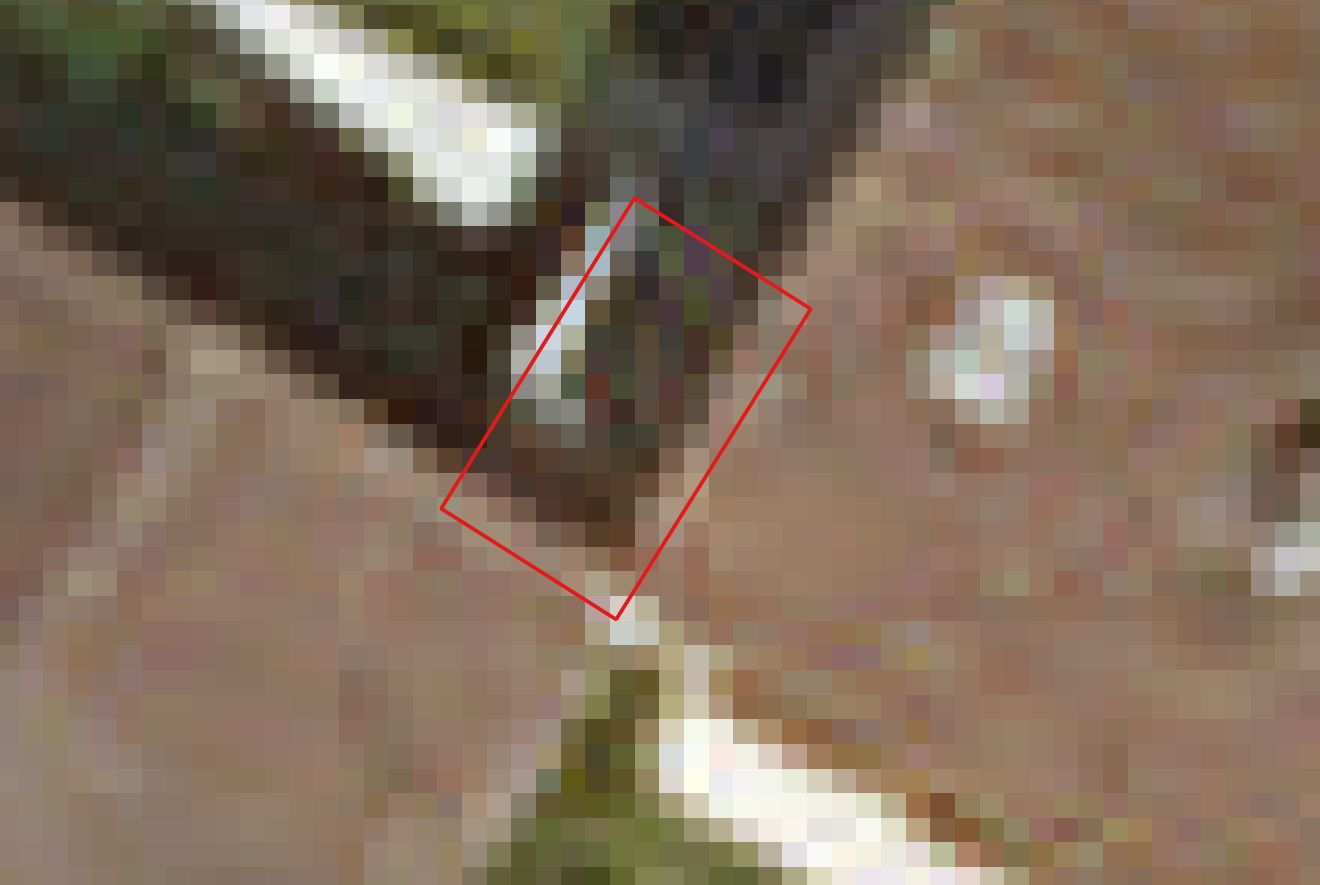
\includegraphics[width=.24\textwidth]{images/raster/Building_Errors/altimetric}}}
                    \end{subfloatrow}
                }
                {
                    \renewcommand\figurename{}
                    \renewcommand{\thefigure}{(\roman{SubFigCounter})}

                    \caption{Building errors samples.}\label{fig::bul_err}
                    \refstepcounter{SubFigCounter}
                }
                \ffigbox[\FBwidth]
                {
                    \begin{subfloatrow}[4]
                        \captionsetup{labelformat=brace, justification=raggedright}
                        \ffigbox[\FBwidth]{\caption{Under Segmentation: Two facets or more grouped into one.}\label{fig::under_fac}}{\fbox{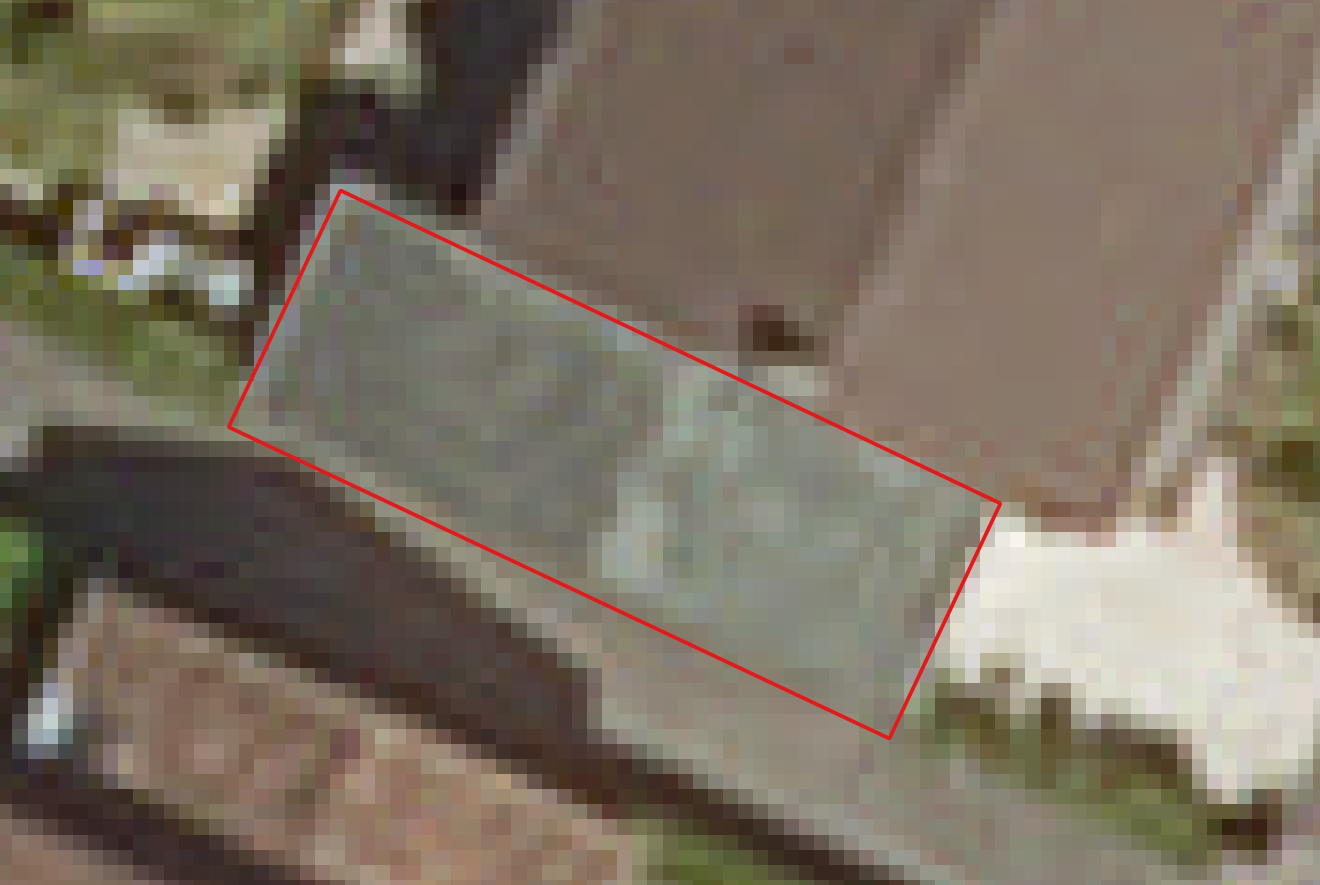
\includegraphics[width=.24\textwidth]{images/raster/Facet_Errors/under_segmentation}}}
                        \ffigbox[\FBwidth]{\caption{Over segmentation: One facet segemented into two or more facets.}\label{fig::over_fac}}{\fbox{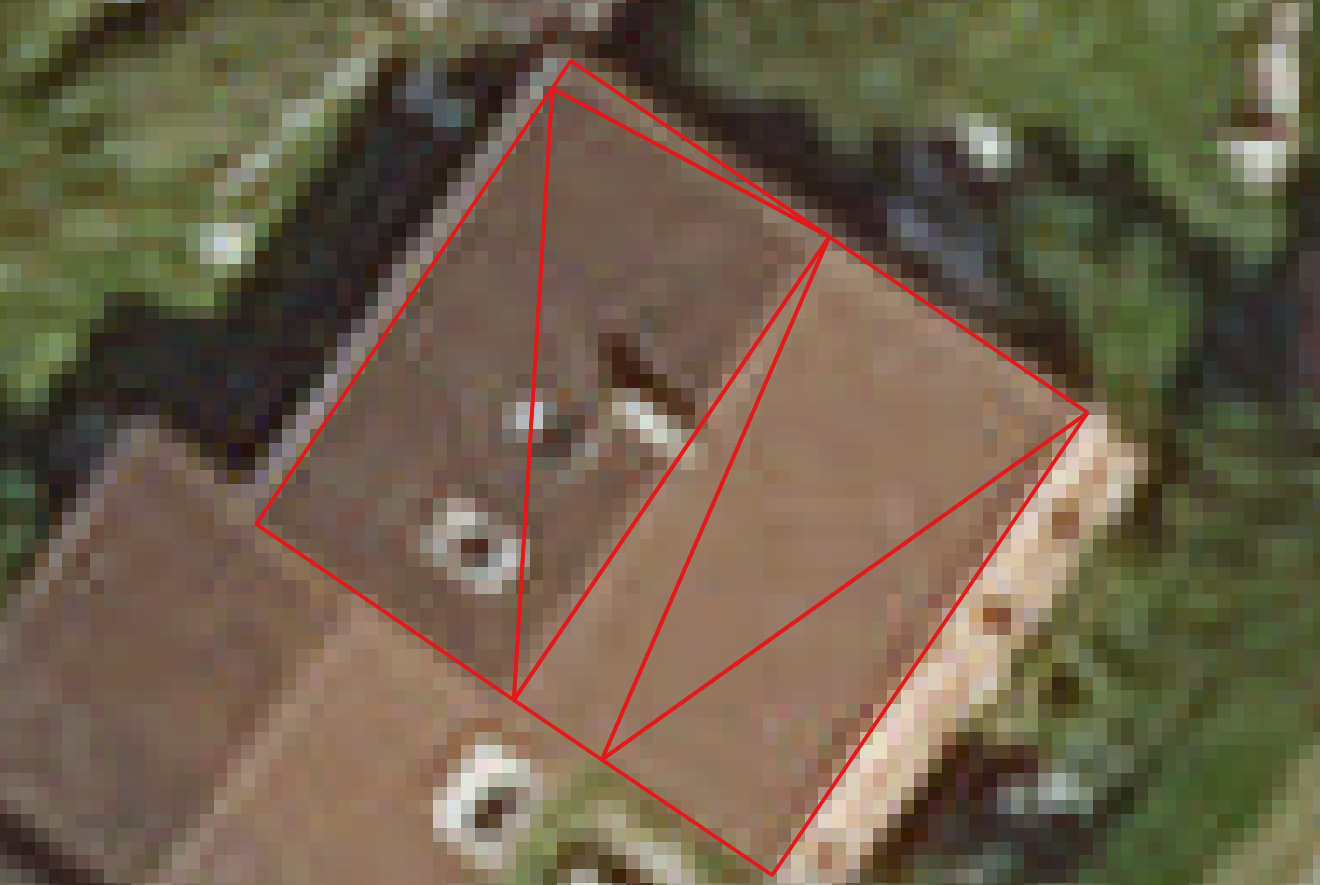
\includegraphics[width=.24\textwidth]{images/raster/Facet_Errors/over_segmentation}}}
                        \ffigbox[\FBwidth]{\caption{Mis Segmentation: Facet edges do not correspond to real ones.}\label{fig::mis}}{\fbox{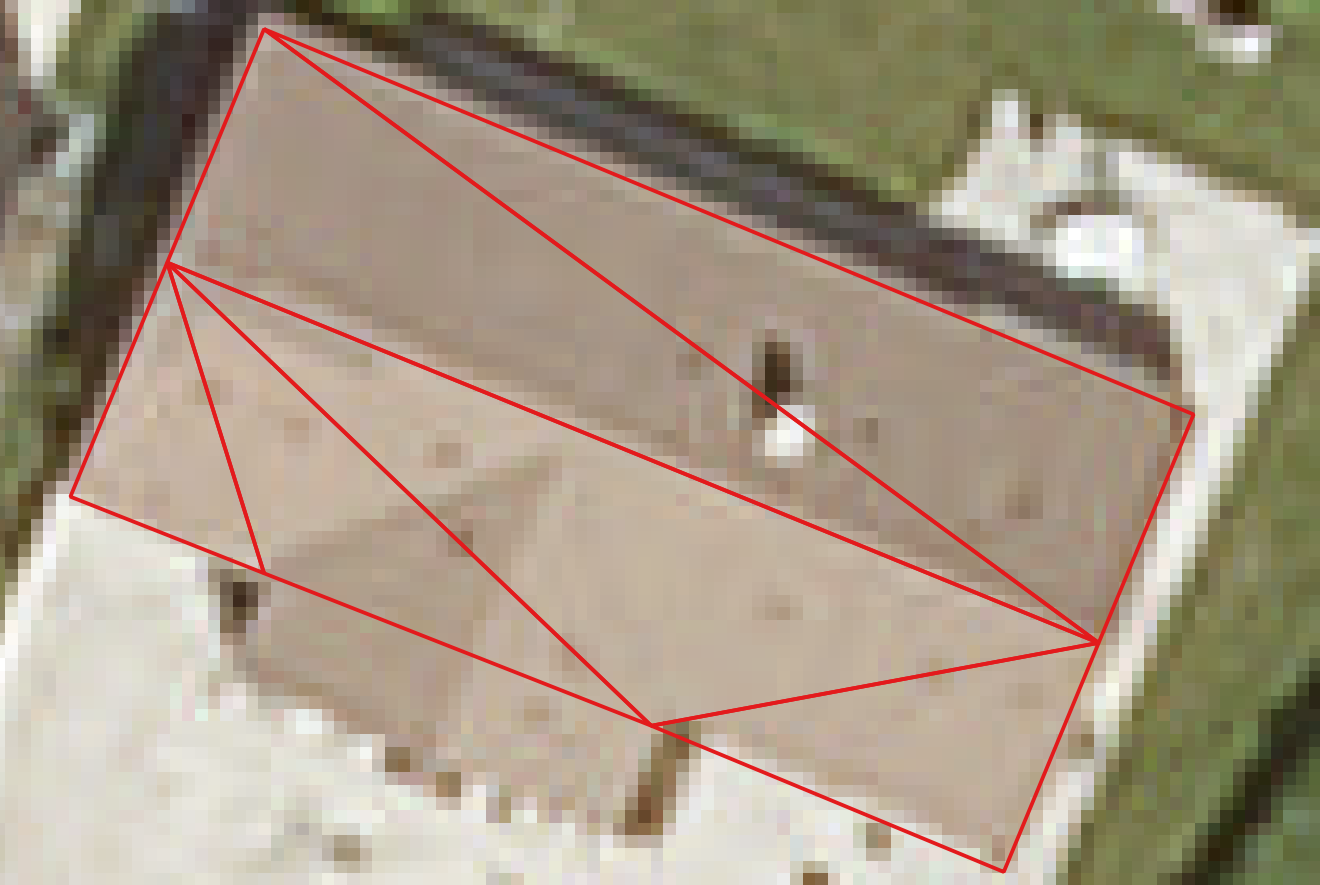
\includegraphics[width=.24\textwidth]{images/raster/Facet_Errors/mis_segmentation}}}
                        \ffigbox[\FBwidth]{\caption{Slope: Wrong facet slope.}\label{fig::slope}}{\fbox{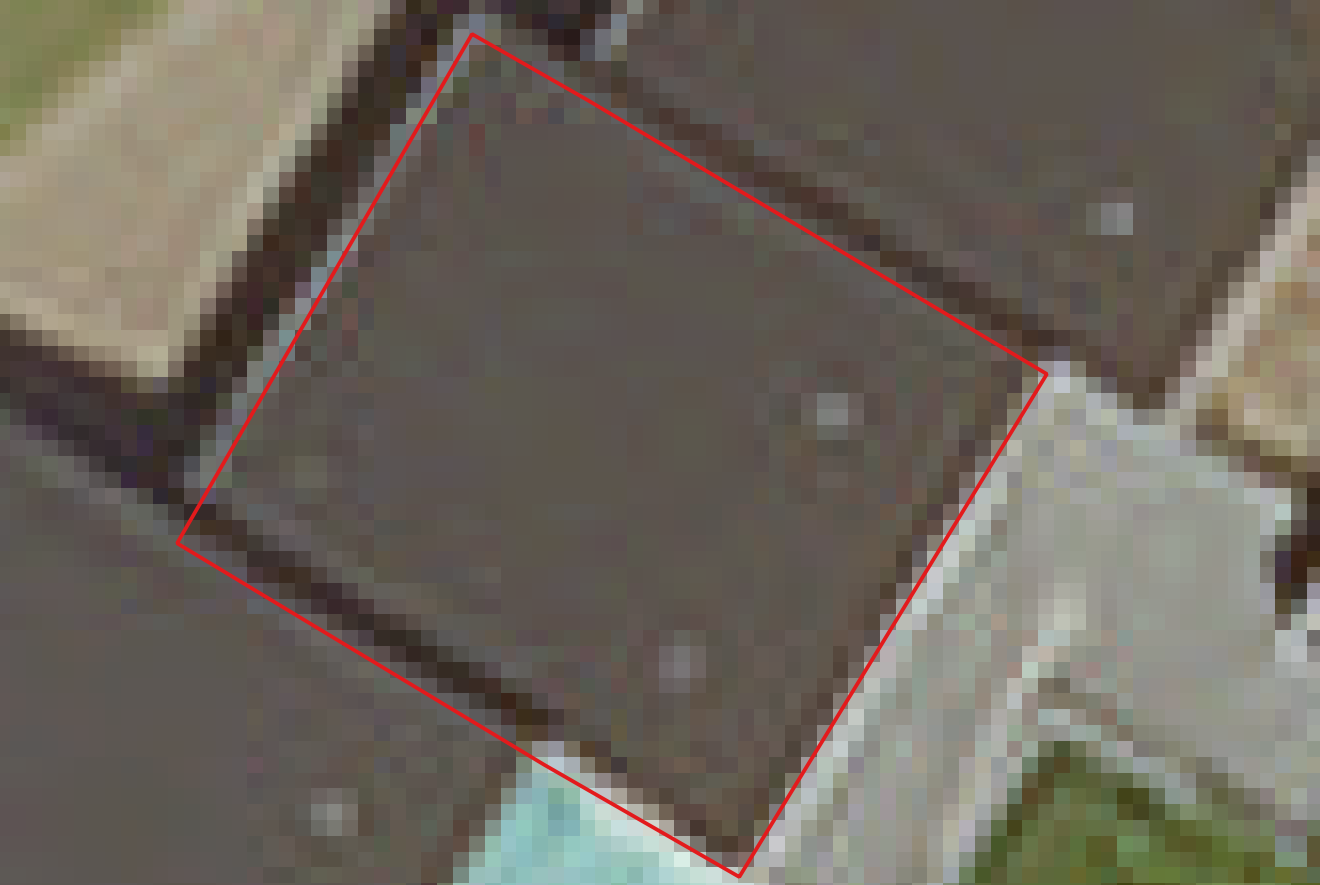
\includegraphics[width=.24\textwidth]{images/raster/Facet_Errors/slope}}}
                    \end{subfloatrow}
                }
                {
                    \renewcommand\figurename{}
                    \renewcommand{\thefigure}{(\roman{SubFigCounter})}

                    \caption{Facet errors samples.}\label{fig::fac_err}
                    \refstepcounter{SubFigCounter}
                }
            }
            {
                \addtocounter{figure}{-3}
                \caption{\label{fig::samples}Error taxonomy illustration.}
            }
        \end{center}
    \end{figure}

    Les erreurs ci-répértoriées sont représentées dans une carte heuristique \textit{c.f.} Figure~\ref{fig::mindmap_errors}. Les statistiques de ces erreurs sont résumées dans la Tableau~\ref{tab::label_stats}.


    \begin{figure}[h!]
        \begin{center}
            \includestandalone[mode=buildnew, width=\textwidth]{mind_map}
            \caption{\label{fig::mindmap_errors} Carte mentale qui résume la taxonomie d'erreur établie.}
        \end{center}
    \end{figure}

    \begin{itemize}
        \item Les erreurs répertoriées dans~\cite{Michelin2013} peuvent être comparée à l'étiquetage que nous avons introduit. L'erreur de bâtiment inexistant est englobée par l'erreur bâtiment modifié. L'Occlusion Végétale représente une partie des erreurs d'occlusion possible que nous avons détectées. Les deux rendent modèles non qualifiables. L'étiquette Cours Manquante n'existe pas dans notre base de données mais peut être considérée comme une erreur de bâtiment. Emprinte inexacte et Contour Erroné font partie de l'étiquette Empreinte Imprécise. On ne cosidère pas Toit Imprécis comme une erreur \emph{atomique}: elle serait causée en grande partie par Segmentation Imprécise. La Sur Segementation et la Sous Segmentation peuvent concerner les bâtiments comme les facettes: elles sont subdivisées dans notre cas entre les deux familles d'erreurs.
        \item Nous retrouvons les différentes qualités définis dans l'étude menée par~\cite{Boudet2006} avec un niveau de quantisation plus développé ($4$ contre $11$ actuels). Dans le modèle actuel, on peut déduire une confiance dans le modèle, en général, à partir des degré de confiance dans l'existance des erreurs atomiques.
    \end{itemize}

    \begin{table}[H]
        \centering
        \caption{\label{tab::label_stats} Label statistics over the $502$ building dataset.}
        \begin{tabular}{x{4cm} | x{3cm} | x{3cm} | x{3cm} | x{3cm}}
            \toprule
            \multicolumn{1}{c|}{\textbf{Error Class}} & \textbf{Occurence probability} & \textbf{Subclass} & \textbf{Class conditionnal occurence probability} & \textbf{Absolute occurence probability} \\
            \midrule
            \multirow{4}{*}{Unqualified Buildings} & \multirow{4}{*}{$0.0876$} & Half Building & $0.8636$ & $0.0757$ \\
            \cline{3-5}
                &                   & Changed Building & $0.0455$ & $0.0040$ \\
            \cline{3-5}
                &                   & Occlusion & $0.0455$ & $0.0040$ \\
            \cline{3-5}
                &                   & Unknown & $0.0455$ & $0.0040$ \\
            \midrule
            \midrule
            \multirow{4}{*}{Building Error} & \multirow{4}{*}{$0.2408$} & Over Segmentation & $0.1365$ & $0.0328$\\
            \cline{3-5}
                &                   & Under Segmentation & $0.4177$ & $0.1006$ \\
            \cline{3-5}
                &                   & Footprint & $0.4839$ & $0.1165$ \\
            \cline{3-5}
                &                   & Altimetric & $0.0165$ & $0.0040$ \\
            \midrule
            \midrule
            \multirow{4}{*}{Facet Errors} & \multirow{4}{*}{$0.81657$} & Over Segmentation & $0.8830$ & $0.7203$ \\
            \cline{3-5}
                &                   & Under Segmentation & $0.0842$ & $0.0687$ \\
            \cline{3-5}
                &                   & Mis Segmentation & $0.0806$ & $0.0657$ \\
            \cline{3-5}
                &                   & Slope & $0.0327$ & $0.0267$ \\
            \bottomrule
        \end{tabular}
    \end{table}


    \section{Méthode proposée}
    \section{Conclusion et perspectives}

    \bibliographystyle{abbrv}
    \bibliography{references}
\end{document}
